\renewcommand*\descriptionlabel[1]{\hspace\leftmargin$#1$}
\setcounter{tocdepth}{5}
\setcounter{secnumdepth}{5}




In the literature review, I showed how various papers have employed different codes, reactors, reprocessing methods, and tracking of DNPs. I also discussed how a reason for employing both continuous and batchwise reprocessing could be to ensure the mass in the reactor remains fairly constant. In this chapter, I will discuss the methodology used for the Serpent2 MSBR model used to generate results, the different reprocessing methods, mass balancing, and delayed neutron precursors in this work.
More specifically, I will describe in detail two different approaches for batchwise reprocessing which have been implemented in SaltProc, the tool used in this work to handle batchwise reprocessing \cite{rykhlevskii_saltproc_2018}. I will then give a summary of the two approaches and provide estimates for the expected error and computational costs compared to continuous methods.
After that, I will then discuss three different continuous reprocessing methods.
I will discuss several approaches which can be implemented for one of these methods.
Finally, I will provide information on the mass balancing and the effects of delayed neutrons on depletion results.


\section{Serpent MSBR Model}

The results generated in this work come from the MSBR, particularly the model developed by Rykhlevskii \cite{rykhlevskii_advanced_2018}. The geometry of the model has remained unchanged, while the reprocessing has been overhauled using the continuous reprocessing functionality previously undocumented in Serpent2. %Previously, SaltProc's batchwise reprocessing was used, but the continuous reprocessing in Serpent2 is incorporated in this work.

\subsection{Reprocessing Structure}
\label{s:decay-tank}

There are two different reprocessing schemes developed in this work. Both schemes follow the MSBR reprocessing scheme, and vary how refueling functions. The first method matches the method of Rykhlevskii, where the uranium-233 feed is treated as equivalent to the protactinium-233 removal rate. In this case, the average uranium-233 feed rate from Rykhlevskii is used over the entire simulation time \cite{rykhlevskii_advanced_2018}. A simplified overview of this scheme can be seen in Figure \ref{fig:spmatchrepr}.


\begin{figure}[H]
  \centering
  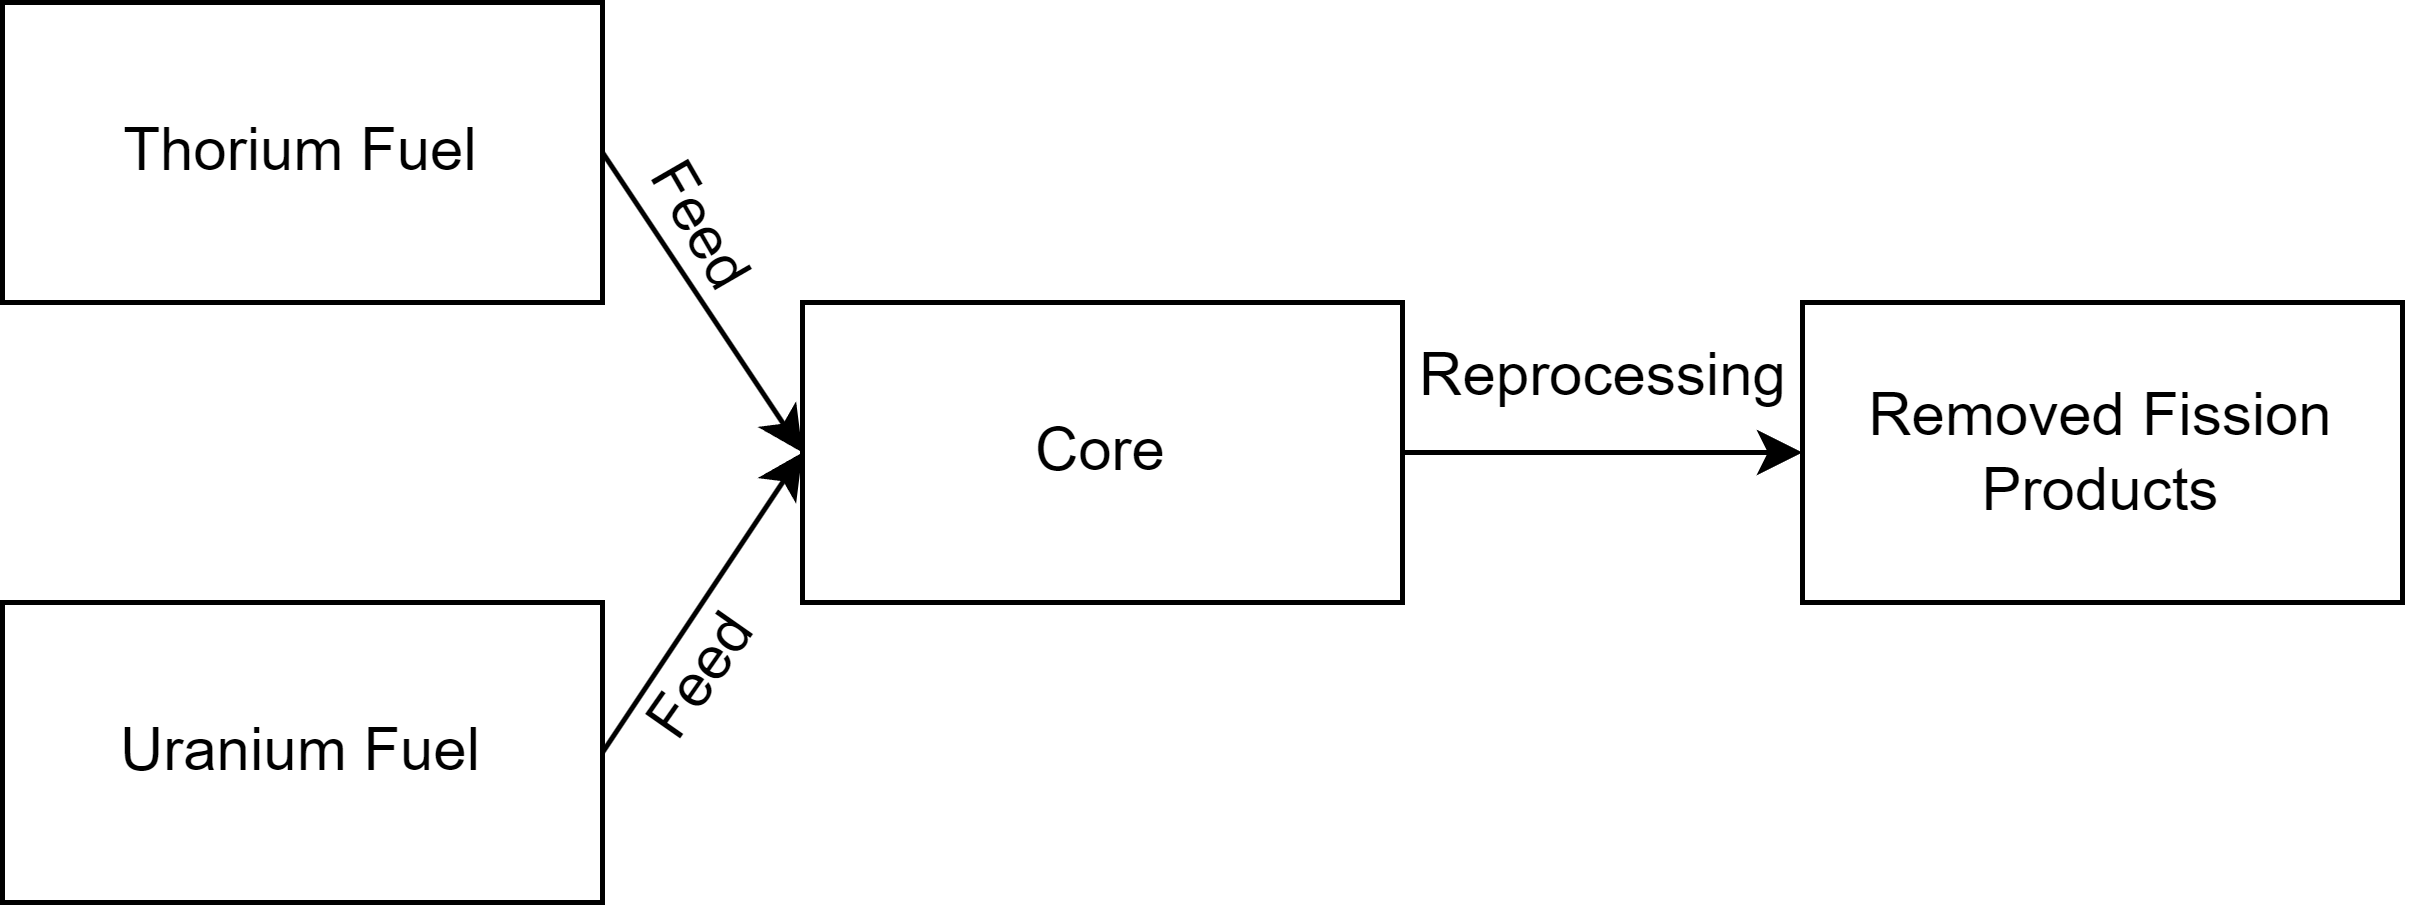
\includegraphics[scale=0.15]{images/sp-match-repr-scheme.png}
  \caption{Simplified reprocessing scheme based on SaltProc.}
   \label{fig:spmatchrepr}
\end{figure}

The second reprocessing scheme reflects the physical MSBR model, and instead uses a protactinium decay tank. From this tank, any bred uranium is continuously removed and sent back to the core, which is the intended design scheme for the MSBR \cite{robertson_conceptual_1971}. A simplified version of the phyiscally realistic uranium feed can be seen in Figure \ref{fig:nonspmatchrepr}.

\begin{figure}[H]
  \centering
  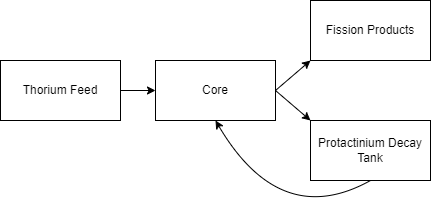
\includegraphics[scale=0.15]{images/phys-repr-scheme.png}
  \caption{Simplified reprocessing scheme based on the phyiscal MSBR processes.}
   \label{fig:nonspmatchrepr}
\end{figure}

Overall, it can be anticipated that the two methods will be approximately equal at steady state, because at steady state the assumption by Rykhlevskii that the uranium input is the same as the protactinium output will be valid. However, there are expected to be differences for the first several months of operation, as the half life of protactinium-233 is on the order of one month, and the initial decrease in fissile material will impact reactor performance. Thus, the uranium feed will take some time before it is providing a steady source of fissile material to the core. Furthermore, the reactor physics will be different, which is important when considering the safety of the reactor.







\section{Batchwise Reprocessing in the MSBR}
\label{s:batch-generic}

As previously mentioned in Section \ref{s:SP-repr}, SaltProc has two different versions which use two different batchwise reprocessing approaches.
These approaches are the bulk batchwise approach, used in version 0.1 of SaltProc, and the steady batchwise approach, used in version 0.3 of SaltProc. In the next two subsections, I will describe each of these approaches and how they differ.

%SaltProc is used to handle batchwise reprocessing in this work because it provides a batchwise reprocessing scheme which can be customized fairly easily.
%SaltProc is used to handle batchwise reprocessing in this work because it uses Serpent2, which has built-in continuous reprocessing; comes with the MSBR geometry in Serpent2 as an example; and has multiple versions.
%Of these different versions of SaltProc, they have slightly different methods in how the depletion data is stored as well as how reprocessing rates are calculated.
%However, the two versions of interest are version 0.1 and 0.3, which use different batchwise reprocessing approaches.
%These two different approaches are referred to here as the "bulk" approach and the "steady" approach.
%which 
%an accurate model of the MSBR, uses Serpent2 for transport and depletion calculations, and because it provides

\subsection{Bulk Reprocessing Approach}

%SaltProc version 0.1 was the first full version of SaltProc publicly released, and provides all the functionality necessary for modeling the MSBR with batchwise reprocessing.
%Using this version, Rykhlevskii uses three day depletion steps and does not perform fractional reprocessing at each step, instead performing reprocessing according to the cycle times \cite{rykhlevskii_advanced_2018}.
%This approach is termed as the "bulk" approach to batchwise reprocessing, and is explained in more detail below. This is the same approach used by Gehin and Powers for an analysis of the MSBR \cite{gehin_liquid_2016}.

The bulk approach operates by removing 100\% of the target once a cycle time, or time it takes for a given element to be completely removed, is met or exceeded.
For example, consider a simulation with a three day depletion step size. An element with a 30 day cycle time would have no reprocessing during the first 27 days, then full 100\% removal of the target at the 30 day mark. This works well for reactor processes which are performed batchwise, such as adding uranium to the reactor which can be performed as a batch process. However, this approach is not ideal for approximating online reprocessing, as it does not capture physics that occur due to frequent reprocessing.

For the refueling of the reactor, the thorium feed rate was set to maintain constant mass in the reactor. This means that after a bulk removal of a large amount of fission products, there will be an equivalent amount of thorium added. Using a steady state approximation, the uranium feed rate is set to be equivalent to the protactinium removal rate at each time step. Specifically, the protactinium is removed first, and then the same mass of fresh uranium is added. This carries an implicit assumption that there is already a backlog of decayed protactinium which has transmuted into uranium which is ready to be pumped back into the core. Both the thorium feed and protactinium to uranium refueling processes occur every 3 days. These refueling rates can be seen in Figures \ref{fig:Th-feed-v1} and \ref{fig:U-feed-v1}, which are recreated from the data from Rykhlevskii \cite{rykhlevskii_advanced_2018}.

% Include figure of U and Th feed rates over time.

\begin{figure}[H]
  \centering
  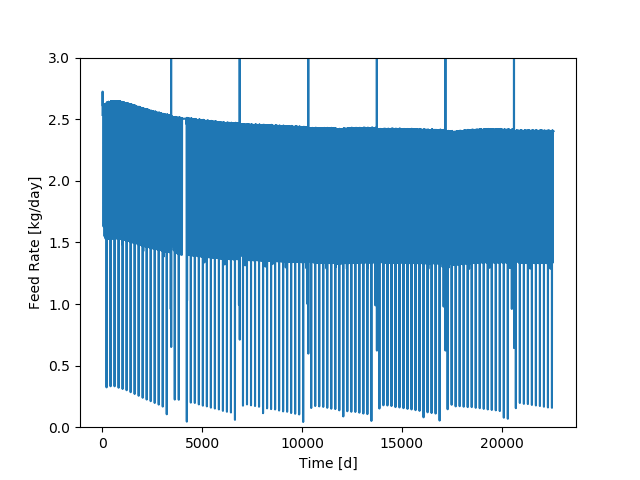
\includegraphics[scale=0.75]{images/Th232rem_massv01.png}
  \caption{Thorium feed rate in the MSBR as a function of time while using bulk batchwise reprocessing \cite{rykhlevskii_advanced_2018}.}
   \label{fig:Th-feed-v1}
\end{figure}

\begin{figure}[H]
  \centering
  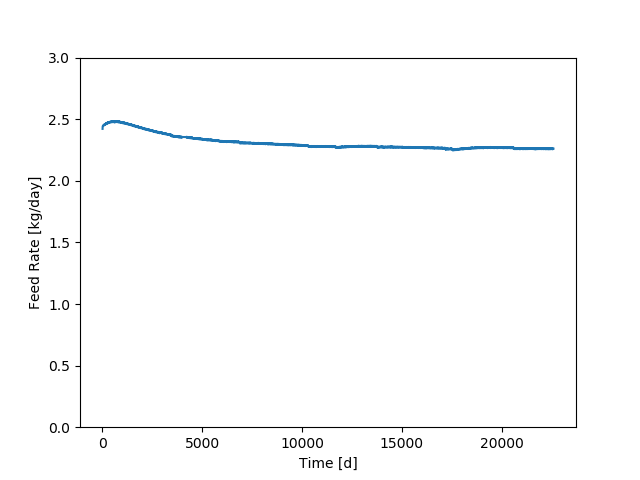
\includegraphics[scale=0.75]{images/Pa233rem_massv01.png}
  \caption{Uranium feed rate in the MSBR as a function of time while using bulk batchwise reprocessing \cite{rykhlevskii_advanced_2018}.}
   \label{fig:U-feed-v1}
\end{figure}

The large jumps in the thorium feed rate are due to the bulk removal of rubidium, strontium, caesium, and barium; this causes jumps in the thorium feed rate because the thorium feed rate in this version of SaltProc is based on mass balancing.
Removing a large amount of fission products results in that mass being replaced by thorium.
This also leads to spikes in the effective multiplication factor, as the removal of the fission products inserts more reactivity than the addition of thorium removes \cite{rykhlevskii_advanced_2018}. The uranium feed rate is smooth because it is based purely on the outflow of protactinium and does not fluctuate like the thorium, which is the only external feed in the MSBR system. The average thorium-232 feed rate is 2.38 kg/day over 20,000 days, while the average uranium-233 feed rate is 2.31 kg/day over the same 20,000 days. These average values are used as the baseline for the feed rates in the rest of this work.

\subsection{Steady Reprocessing Approach}
\label{s:steady}

%SaltProc version 0.3 includes an example MSBR which users can run as soon as SaltProc is installed, though some of the run parameters such as neutrons per generation and run time have to be altered to generate a more valid model. This model also uses 3 day steps, but instead of performing the batch removal only at the cycle time value, this model removes a fraction every 3 days, which is called the "steady" approach for batchwise reprocessing.
Steady batchwise removes a fraction of the target at each depletion time step rather than 100\% removal at certain time steps.
For example, a 30 day cycle time would result in 10\% removal every 3 days. This more accurately models online reprocessing, which is primarily what the MSBR employs in its reprocessing scheme. However, this steady version of SaltProc also makes some minor changes to the reprocessing scheme by adding in efficiency terms. These changes act as a multiplier on the reprocessing constant, where 100\% efficiency makes no change and 0\% makes the reprocessing constant become 0, as shown in Equation \eqref{eq:batchwise_rem_eff}. The changes used in this work to replicate the work by Rykhlevskii are as follows: xenon uses 91.2\% removal over three days instead of 100\%, krypton uses 91.5\% removal over three days instead of 100\%, protactinium uses 9.5\% removal over three days instead of 100\%, and the discard of rubidium, strontium, caesium, and barium have a removal of 0.9\% over three days instead of 0.09\% \cite{rykhlevskii_fuel_2020, rykhlevskii_saltproc_2018}. These rates come from the cycle times in Table \ref{tab:msbr_cycle_times} and Equation \eqref{eq:batchwise_rem_eff}.

The reactor refueling in steady batchwise reprocessing is performed slightly differently from the bulk batchwise method as well. The former assumes a constant ratio for the refueling quantities of uranium and thorium. The net refueling for each 3 day depletion step is set to maintain the mass of the system. Thus, the average values of 2.38 kg/day and 2.31 kg/day for thorium-232 and uranium-233, respectively, are used to determine the ratio of uranium to thorium which is implemented.

Figures \ref{fig:Th-feed-v3} and \ref{fig:U-feed-v3} show the refueling rate of thorium-232 and uranium-233, respectively, using a depletion step size of 3 days over a net depletion simulation time of 90 days. The average feed rates of the thorium-232 and uranium-233 are 1.24 and 1.21 kg/day. The reasons for the difference are because the smaller efficiencies cause less mass loss, a shorter time frame is covered, and the protactinium removal is much less, resulting in a much smaller uranium-233 feed.

\begin{figure}[H]
  \centering
  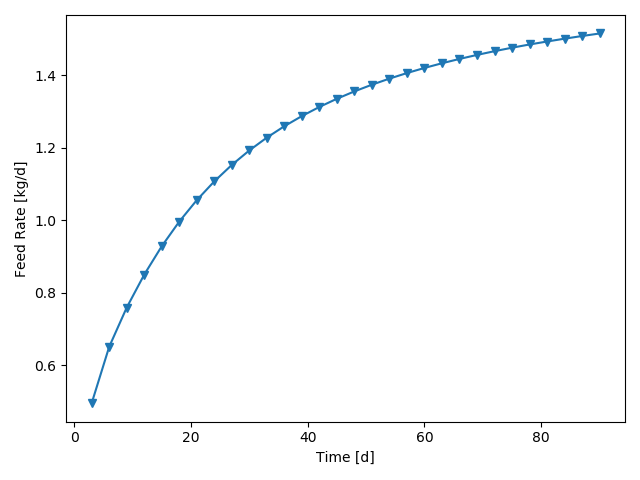
\includegraphics[scale=0.75]{images/feed_Th232_3d_90d.png}
  \caption{Thorium feed rate with a depletion time step of 3 days in the MSBR as a function of time while using steady batchwise reprocessing.}
   \label{fig:Th-feed-v3}
\end{figure}

\begin{figure}[H]
  \centering
  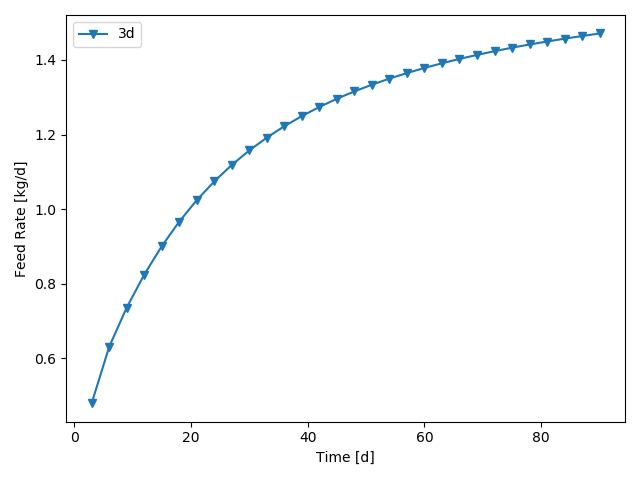
\includegraphics[scale=0.75]{images/feed_U233_3d_90d.png}
  \caption{Uranium feed rate with a depletion time step of 3 days in the MSBR as a function of time while using steady batchwise reprocessing.}
   \label{fig:U-feed-v3}
\end{figure}

%Additionally, this version of SaltProc uses the PyTables Python package for handling the hdf5 data files. The data files are structured similarly to v0.1 of SaltProc, but instead of atom density they use mass, which makes analysis of the files slightly more user friendly.

\subsection{Batch Approaches Summary}
\label{s:batch-sum}

To compare the different batchwise approaches, there are several key parameters to keep in mind. These include the approach used, which can be either bulk or steady for this work; the time step $\Delta t$, which is the simulated depletion time step used; and the cycle time $T_{cyc}$, which is inversely proportional to the rate at which a target is removed. 
The step removal for both steady and bulk can then be calculated, where the step removal is the fraction of the target removed at each depletion time step.
%For both steady and bulk, the step removal can then be calculated, which is the fraction of the target removed at each depletion time step. 
Additionally, for the steady, the fractional removal rate can be calculated. This is just the step removal in per second units. Comparisons of these values for various parameters can be seen in Table \ref{tab:batch_methods}.

\begin{table}[H]
\renewcommand{\arraystretch}{1.25}
\caption{Batchwise Reprocessing Methods}
\label{tab:batch_methods}
\begin{center}
\begin{tabular}{ c | c | c | c | c }
 \hline
        Approach & $\Delta t$ $[s]$ & $T_{cyc}$ $[s]$ & Fractional Removal Rate [s$^{-1}$] & Step Removal\\
 \hline
 \hline
        Bulk & 1 & 20 & - & \, 0/1$^{*}$\\
        Bulk & 10 & 20 & - & \, 0/1$^{*}$ \\
        Bulk & 40 & 20 & - & 1 \\
        Steady & 1 & 20 & 0.05 & 0.05\\
        Steady & 10 & 20 & 0.05 & 0.5\\
        Steady & 40 & 20 & 0.025 & 1\\
 \hline
\end{tabular}
\end{center}
\end{table}
        \begin{center}
\footnotesize{$^{*}$ Bulk removal is 0 until the depletion step is equal to the cycle time, at which point it removes 100\%.}\\
        \end{center}
        
Table \ref{tab:batch_methods} reflects the information shown in Figure \ref{fig:bulk_repr_cnst}, which shows the fractional removal rate at each depletion time step. The table shows how the bulk method will only remove 100\% at the cycle time, and otherwise removes nothing. Additionally, the bulk method will remove 100\% as soon as possible if the depletion step size, $\Delta t$, is larger than the cycle time, $T_{cyc}$. 

The table also describes how the steady method fractional removal is constant up until the depletion step size becomes larger than the cycle time, at which point the removal at each step is 100\%, causing the steady method to then be equivalent to the bulk method. However, for shorter times, the steady method allows for a consistent fractional removal rate by adjusting the removal at each step.


\begin{figure}[H]
  \centering
  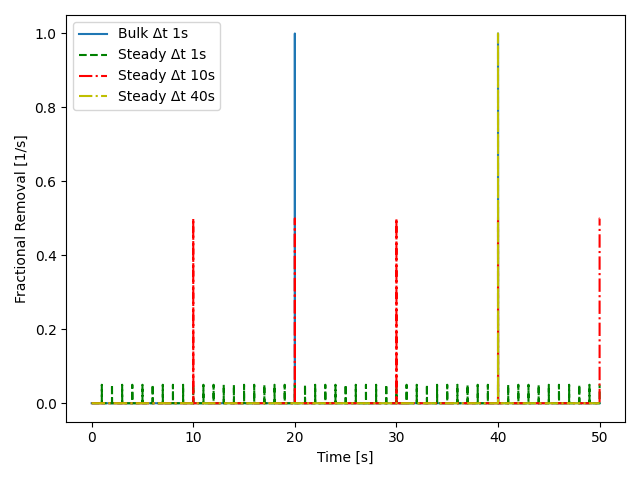
\includegraphics[scale=0.75]{images/bulk-compare-cycles.png}
  \caption{Plot showing how bulk and steady batchwise reprocessing removal works as a function of time for an example with a cycle time of 20 seconds.}
   \label{fig:bulk_repr_cnst}
\end{figure}

Figure \ref{fig:bulk_repr_cnst} shows an example fractional removal scheme for a fission product with a cycle time of 20 seconds. The bulk method simply extracts 100\% of the product every 20 seconds, no matter how small the depletion step size is. The steady method removes some fraction every depletion step, which allows a semi-continuous process as the depletion step size becomes smaller and smaller. This can be seen in how a 10 second depletion step results in 50\% removal every 10 seconds, whereas a 1 second step allows for 5\% removal per depletion step.


% Add comparison of batch/steady for matrix of possible combinations. 

%\begin{figure}[H]
%  \centering
%  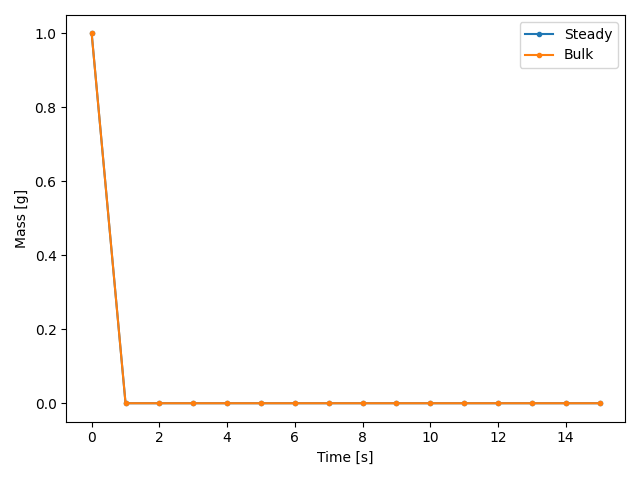
\includegraphics[scale=0.75]{images/batch-steady-identical-compare.png}
%  \caption{Plot showing how bulk and steady batchwise reprocessing are identical in the cases %where the cycle time is shorter than or equal to the depletion step size.}
%   \label{fig:bulk_repr_comp}
%\end{figure}

A useful piece of information to note is that if the cycle time is shorter than or equal to the depletion step size, then the steady and bulk batchwise methods will be identical to each other.
%This is demonstrated in Figure \ref{fig:bulk_repr_comp}, which shows a simple model case with 1 second depletion steps and 1 second cycle times for an imaginary isotope. 
For the MSBR simulation, this means that there will be no mass differences due to reprocessing in the noble metals, gasses, and protactinium while using a three day depletion time step, which is longer than or equal to the cycle time for each of those groups. % reprocessing will remain the same for either batchwise method employed.
However, the longer cycle time groups, such as the rare earths and volatile fluorides, have cycle times which are 10-20 times longer than the depletion step size. These elements will have differences between both methods. As a result, the full reactor system will have elements with varying levels of error.

Figure \ref{fig:bulk_repr_diff} shows a simulation of this for a situation where an isotope is generated at a rate of 1 gram per second, and is simulated with some combination of cycle time and depletion step size where the depletion step size is smaller than the cycle time.

\begin{figure}[H]
  \centering
  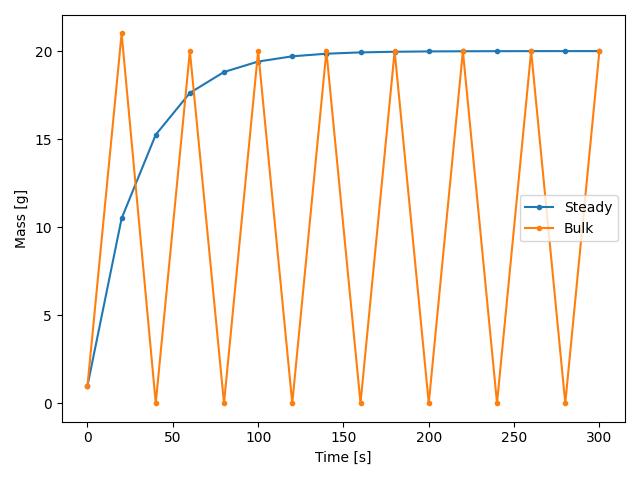
\includegraphics[scale=0.75]{images/batch-40-20.png}
  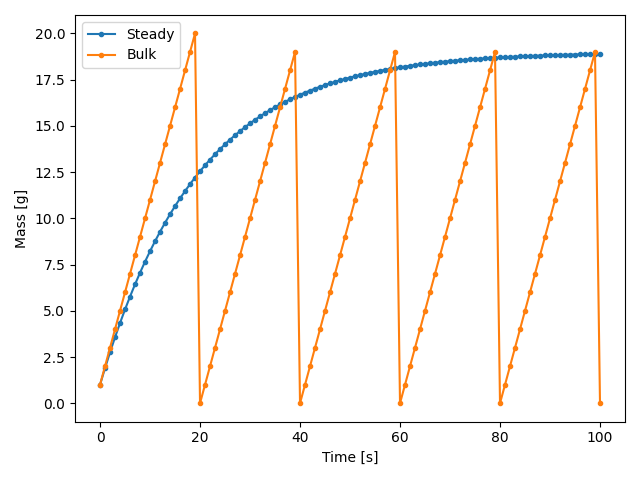
\includegraphics[scale=0.75]{images/batch-20-1.png}
  \caption{Plot showing how bulk and steady batchwise reprocessing are different while the cycle time is longer than the depletion step size. In this system, the element has a 40 second cycle time and 20 second depletion step (top) and a 20 second cycle time with a 1 second depletion step (bottom).}
   \label{fig:bulk_repr_diff}
\end{figure}

One interesting aspect to note from this figure is that the steady method approaches a steady state value which is at the peak of the bulk method. This result can be confirmed by checking that the solutions for both the steady and bulk methods are valid. To check the solution, the 40 second cycle time and 20 second depletion step will be used. 

For the bulk method, after 100\% removal following the first cycle time, or 40 seconds, the mass then oscillates between 20 and 0 grams. 
This is consistent with the expected result, since 20 grams are generated over 20 seconds while every 40 seconds there is 100\% removal. 

For the steady method, the initial mass of 1 gram gains 20 grams over 20 seconds, yielding 21 grams. However, the steady removal then requires removal of 50\%, previously discussed and shown in Figure \ref{fig:bulk_repr_cnst}. This 50\% removal then drops the mass to 10.5 grams. 20 more grams are added to this value and 50\% is removed again, continuing iteratively. This can then be re-written as an infinite sum in order to determine the steady state solution. The first three iterations are shown in Equations \eqref{eq:ss-mass-p1} and \eqref{eq:ss-mass-p2}, where the value of 20 is the mass added during each depletion step and the value of 0.5 is the fractional removal performed each depletion step. 
%In the generic form, the $C$ term represents the gain per second, $\Delta t$ is the depletion step size, and $T_{cyc}$ is the cycle time.

%\begin{equation} \hfill 
%m_{n+1} = (m_n + C \Delta t) (1 - \frac{\Delta t}{T_{cyc}})
%\hfill\label{eq:ss-mass-p5-steady-generic} \end{equation}

\begin{equation} \hfill 
m_{ss} = \left( \left( \left(N_0+20 \right) \left(\frac{1}{2} \right)+20 \right)\left(\frac{1}{2} \right)+20 \right)\left(\frac{1}{2} \right) + ...
\hfill\label{eq:ss-mass-p1} \end{equation}

\begin{equation} \hfill 
m_{ss} = \frac{1}{2}^3 N_0 + \frac{1}{2}^3 (20) + \frac{1}{2}^2 (20) + \frac{1}{2} (20) + ...
\hfill\label{eq:ss-mass-p2} \end{equation}

Continuing this form infinitely yields Equation \eqref{eq:ss-mass-p3}, where the infinite sum yields 1, resulting in a net value of 20, the result of which is unaffected by the initial mass of the isotope and instead depends on the generation and reprocessing rates.

\begin{equation} \hfill 
m_{ss} = 20 \sum_{n=1}^\infty \frac{1}{2}^n 
\hfill\label{eq:ss-mass-p3} \end{equation}

In order to generate a generic form for this equation, a short derivation is required, which is provided in Appendix A. From this derivation, the mass at the $n+1^{th}$ step is given by Equation \eqref{eq:nplusone-gen}.

\begin{equation} \hfill 
m_{n+1} = \left[ \left(m_n + \frac{C}{\lambda - \lambda_r} \right)e^{-(\lambda - \lambda_r) \Delta t} + \frac{C}{\lambda - \lambda_r} \right] \left(1 - \Delta t \lambda_r \right),
\hfill\label{eq:nplusone-gen} \end{equation}

% Add generic form (x added per second, y removal rate)A more generic form for the case of a constant rate of change over each depletion step can be seen in Equation \eqref{eq:ss-mass-p4}. 
In this equation, $C$ represents the gain terms in the Bateman equation, $\Delta t$ represents the depletion step size, $\lambda$ represents the loss terms in the Bateman equation, and $\lambda_r$ represents the reprocessing constant. This equation assumes a constant $C$, $\lambda$, and $\lambda_r$.
This is a reasonable assumption at steady state when the changes over time are negligible. This equation is used to generated the steady state equation as shown in Equations \eqref{eq:ss-mass-p4prev} through \eqref{eq:ss-mass-p4}.

%\begin{equation} \hfill 
%m_{ss} = C \Delta t \sum_{n=1}^\infty \left( 1 - \frac{\Delta t}{T_{cyc}} \right)^n 
%\hfill\label{eq:ss-mass-p4prev} \end{equation}

The $n+1^{th}$ step can be written in the form of a sum over $n$ terms, which allows for the steady state mass to be written as an infinite sum

\begin{equation} \hfill 
m_{ss} =  \frac{C}{\lambda - \lambda_r} \left(e^{(\lambda - \lambda_r) \Delta t} - 1 \right) \sum_{n=1}^{\infty} \left( \left(1 - \lambda_r \Delta t \right) e^{-(\lambda - \lambda_r) \Delta t} \right)^n.
\hfill\label{eq:ss-mass-p4prev} \end{equation}

This infinite sum is of the more general form

\begin{equation} \hfill 
\sum_{n=1}^\infty \left( x \right)^n = \frac{x}{1-x} \ni |x| < 1,
\hfill\label{eq:ss-mass-p4next} \end{equation}

which has a known converged solution and associated constraint to use that converged solution. I can then rewrite the infinite sum as

\begin{equation} \hfill 
m_{ss} =  \frac{C (e^{(\lambda - \lambda_r) \Delta t} - 1)}{\lambda - \lambda_r}  \left( \frac{\eta}{1 - \eta} \right) \ni \left|\eta \right| < 1,
%m_{ss} =  C \Delta t \left( \frac{T_{cyc}}{\Delta t} - 1 \right) \ni 0 < \frac{\Delta t}{T_{cyc}} < 2
\hfill\label{eq:ss-mass-p4nextprev} \end{equation}

where

\begin{equation} \hfill 
\eta = (1 - \lambda_r \Delta t) e^{-(\lambda - \lambda_r) \Delta t}.
\hfill\label{eq:ss-mass-p4next-simple} \end{equation}

In these equations, $C$ still represents the gain terms in the Bateman equation, $\Delta t$ represents the depletion step size, $\lambda$ represents the loss terms in the Bateman equation including the loss from reprocessing, and $\lambda_r$ represents the reprocessing constant.

The constraint listed in Equation \eqref{eq:ss-mass-p4nextprev} that $\left|\eta \right| < 1$ shows when the equation no longer holds. However, this constraint only shows when the infinite series becomes divergent. The more physical constraint, $0 < \lambda_r \Delta t < 1$ is given in Equation \eqref{eq:ss-mass-p4}, which shows the completed form of the steady state mass. If the depletion step size, $\Delta t$, is equal to zero, then the simulation will never end, as no progress is made. Thus, the concept of steady state does not apply. For any depletion step sizes which are greater than the cycle time, the steady state mass will always be zero, as negative masses are non-physical.

\begin{equation} \hfill 
m_{ss} = \frac{C (e^{(\lambda - \lambda_r) \Delta t} - 1)}{\lambda - \lambda_r}  \left( \frac{\eta}{1 - \eta} \right) \ni 0 < \lambda_r \Delta t < 1
%m_{ss} =  C (T_{cyc} - \Delta t) \ni 0 < \frac{\Delta t}{T_{cyc}} \leq 1
\hfill\label{eq:ss-mass-p4} \end{equation}



Overall, this shows that the steady and bulk batchwise methods have some similarities, but for elements with longer cycle times, the bulk method will experience oscillations whereas the steady method will level off smoothly. Additionally, the average value of the steady method will be higher than the oscillating bulk method. Finally, if I take the limit of Equation \eqref{eq:ss-mass-p4} as the time step approaches zero, Equation \eqref{eq:ss-mass-limit} is generated.

\begin{equation} \hfill 
\lim_{\Delta t \to 0} m_{ss} = \frac{C}{\lambda}
%m_{ss} =  C (T_{cyc} - \Delta t) \ni 0 < \frac{\Delta t}{T_{cyc}} \leq 1
\hfill\label{eq:ss-mass-limit} \end{equation}

This is the same steady state mass as generated from a continuous reprocessing method with the same gain, loss, and reprocessing terms in the Bateman equation.

\subsection{Comparison with Continuous Reprocessing}
\label{s:batch-cont-compare}

\subsubsection{Error Estimation}

The difference between the bulk and steady batchwise reprocessing methods has been demonstrated, though how these methods compare to the continuous reprocessing methods has not been shown. For a simple example comparison, the steady batchwise method will be compared against the direct linear continuous method, which gives the relationship shown in Equation \eqref{eq:ss-mass-p6}. The derivation for this equation can be seen in Section \ref{s:DL}.

\begin{equation} \hfill 
\lambda_r = \frac{1}{T_{cyc}}
\hfill\label{eq:ss-mass-p6} \end{equation}

This comparison will assume there is some isotope which is generated at a constant rate, $C$, and is only removed due to reprocessing. This is a simple case to compare, as there is no parasitic absorption, decay chains, or other more complex physics to treat. Additionally, the impact of the reprocessing differences will be more noticable, as there won't be competing removal effects.


The relevant continuous method equations are given in Equations \eqref{eq:ss-mass-p5} and \eqref{eq:ss-mass-p7}, where the variables are the same as those discussed in Equation \eqref{eq:ss-mass-p4}. Equation \eqref{eq:ss-mass-p5} shows the generic differential equation, while Equation \eqref{eq:ss-mass-p7} shows the mass as a function of time.

\begin{equation} \hfill 
\frac{dm}{dt} = C - \lambda m
\hfill\label{eq:ss-mass-p5} \end{equation}


\begin{equation} \hfill 
m(t) = \left(m_0 - \frac{C}{\lambda} \right) e^{-\lambda t} + \frac{C}{\lambda}
\hfill\label{eq:ss-mass-p7} \end{equation}

Equation \eqref{eq:ss-mass-batch-added} shows the equation for the steady batchwise method mass at the $n+1^{th}$ step. This equation is dependent upon the time step, so several time steps will need to be included in order to properly compare the steady batchwise and direct linear continuous methods.

\begin{equation} \hfill 
m_{n+1} = (C \Delta t + m_n) (1 - \lambda_r \Delta t)
\hfill\label{eq:ss-mass-batch-added} \end{equation}

The previous example is continued here, using a constant rate of 1, an initial concentration of 1, a cycle time of 40 seconds, and a varying depletion step size. The results of this comparison can be seen in Figure \ref{fig:steady_cont_repr_diff}, which is generated by plotting the masses over time for the given equations. In this figure, the continuous initially has a sharp increase in mass which is more closely matched by the steady batchwise approaches which use larger time steps. However, as the simulation time continues, the smaller time step steady batchwise result has a closer value to the continuous than the larger time step approaches.

\begin{figure}[H]
  \centering
  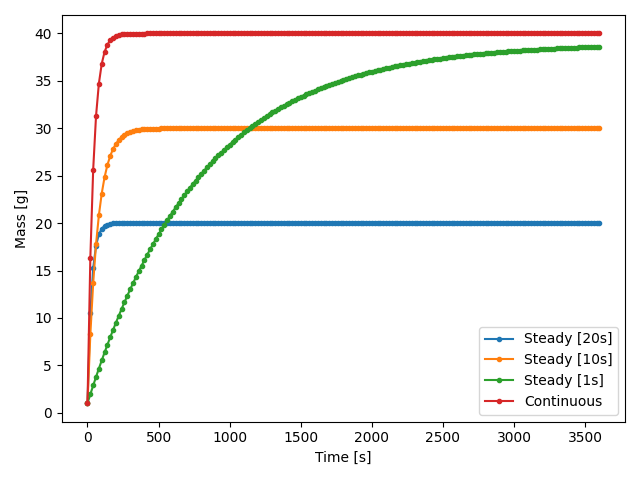
\includegraphics[scale=0.7]{images/dirlin-steady-comp.png}
  \caption{Plot comparing the values of continuous and batchwise reprocessing methods with a 40 second cycle time for an arbitrary nuclide.}
   \label{fig:steady_cont_repr_diff}
\end{figure}

Overall, this figure shows that there are going to be differences between the batchwise and continuous methods, even with a time step which approaches zero. This is due to the differences in the slopes, which can be seen when comparing the continuous and steady for a small time step of one second. However, it can also be seen that the differences at large time values is smaller for shorter time steps and larger for longer time steps when comparing the steady batchwise and continuous methods. From this observation, I provide a derivation for the expected difference between the methods at steady state, with some simplifying assumptions.
%It can be seen in this figure that the direct linear continuous method will result in a steady state result which is different from the steady batchwise method unless the depletion step size is infinitely small.

\begin{equation} \hfill 
m_{ss} = \frac{C}{\lambda}
\hfill\label{eq:ss-mass-cont} \end{equation}

Equation \eqref{eq:ss-mass-cont} shows the steady state mass which will appear when using continuous reprocessing when there is a constant growth term. This can be set equal to the steady batch steady state term in order to solve for the depletion time step needed to match the result from continuous reprocessing at steady state. 
The steady state mass was previously calculated for a time step approaching zero in Equation \eqref{eq:ss-mass-limit}.
In that equation, I showed that the steady state mass calculated using a continuous reprocessing method is equal to the steady state mass cakculated using a steady batchwise reprocessing method when the time step approaches zero.
%The result of this can be seen in Equation \eqref{eq:ss-mass-solve-3}, which reinforces what can be seen in Figure \ref{fig:steady_cont_repr_diff}.

%\begin{equation} \hfill 
%\frac{C}{\lambda} = \lim_{\Delta t \to 0} \left( \frac{C (e^{(\lambda - \lambda_r) \Delta t} %- 1)}{\lambda - \lambda_r}  \left( \frac{\eta}{1 - \eta} \right) \right)
%\hfill\label{eq:ss-mass-solve-3} \end{equation}

Correspondingly, this means that the steady state error associated with implementing the steady batchwise method to approximate a continuous reprocessing scheme is proportional to the magnitude of the depletion step size used. Specifically, as shown in Equations \eqref{eq:ss-err-1} and \eqref{eq:ss-err-4}, the error at steady state due to reprocessing directly scales based on the ratio of the depletion time step and the cycle time. In this work, I treat the error as the normalized difference of the batchwise mass from the continuous mass.

\begin{equation} \hfill 
|E| = \frac{|m_{ss}^{batch} - m_{ss}^{continuous}|}{m_{ss}^{continuous}}
\hfill\label{eq:ss-err-1} \end{equation}

%\begin{equation} \hfill 
%|E| = \frac{|C(T_{cyc} - \Delta t) - CT_{cyc}|}{CT_{cyc}}
%\hfill\label{eq:ss-err-2} \end{equation}

%\begin{equation} \hfill 
%|E| = \frac{|T_{cyc} - \Delta t - T_{cyc}|}{T_{cyc}}
%\hfill\label{eq:ss-err-3} \end{equation}

\begin{equation} \hfill 
|E| = \frac{\lambda}{C} \left| \frac{C}{\lambda}  - \frac{\lambda (e^{(\lambda - \lambda_r) \Delta t} - 1)}{\lambda - \lambda_r}  \left( \frac{(1 - \lambda_r \Delta t) e^{-(\lambda - \lambda_r) \Delta t}}{1 - (1 - \lambda_r \Delta t) e^{-(\lambda - \lambda_r) \Delta t}} \right) \right|
%|E| = \frac{\Delta t}{T_{cyc}} \ni 0 < \frac{\Delta t}{T_{cyc}} \leq 1
\hfill\label{eq:ss-err-4} \end{equation}

An exmaple of this relative error can be seen in Figure \ref{fig:steady_cont_repr_diff}, as the depletion time step to cycle time ratio is exactly 2 for the steady batchwise 20 second step size. Correspondingly, the steady state value is twice is low as the continuous steady state value. Although these equations show only the simplest case of a constant growth, they demonstrate how the important using a small depletion step size is for batchwise methods to generate an accurate result when approximating a continuous scheme.

This method also fits well for complicated interactions which are present in the molten salt reactor model.
As previosuly discussed, for this equation to fit, there are several assumptions which must be made, such as a constant gain and loss terms.
%For this simplified model to fit the MSBR, I make the following assumptions: there is a constant amount of fissile mass in the system (in the case of the MSBR, this is primarily uranium-233, $m_{u233}$), I assume the fission yield ($\gamma$) does not change significantly due to spectral changes over time, and I assume a constant neutron flux ($\phi$).
For this simplified model to fit the MSBR, I make the following assumptions: there is a constant amount of fissile mass in the system, the fission yield does not change significantly due to spectral changes over time, and there is a constant neutron flux.
The equations used to generate the error, particularly Equation \eqref{eq:ss-err-4}, can then be expanded using the variables shown in Equation \eqref{eq:ss-mass-p5-update} and \eqref{eq:ss-mass-p5-steady-update}. The terms in these equations come from the Bateman equation, where $C_i$ is the source term for nuclide $i$, $\phi$ is the neutron flux, $\sigma^{U233}_f$ is the fission cross section of uranium-233, $\gamma_i$ is the fission yield, $N$ is the concentration, $\lambda_{j \rightarrow i, d }$ is the decay constant of nuclide $j$ to nuclide $i$, $\sigma_{j \rightarrow i}$ is the cross section of nuclide $j$ to $i$, $\lambda_i$ is the loss term for nuclide $i$, $\lambda_{i, d}$ is the decay constant for nuclide $i$, $\lambda_{i, r}$ is the reprocessing constant for nuclide $i$, and $\sigma_i$ is the capture cross section for nuclide $i$.

\begin{equation} \hfill 
C_i = \phi \sigma^{U233}_f \gamma_i N_{U233} + \sum_j N_j \left( \lambda_{j \rightarrow i, d }  + \sigma_{j \rightarrow i} \phi \right)
%\frac{dm}{dt} = \phi \sigma_{u233} \gamma m_{u233} - \left( \lambda_{r} + \lambda_d + \phi \sigma \right) m
\hfill\label{eq:ss-mass-p5-update} \end{equation}

\begin{equation} \hfill 
\lambda_i = N_i \left( \lambda_{i, d} + \lambda_{i, r} + \sigma_i \phi \right)
%m_{n+1} = (m_n + \phi \sigma_{u233} \gamma m_{u233} \Delta t) (1 - \Delta t \left(  \lambda_{r} + \lambda_d + \phi \sigma \right) )
\hfill\label{eq:ss-mass-p5-steady-update} \end{equation}

In these equations, the reprocessing constant, $\lambda_r$, is rewritten from its previous form of $\lambda$ because the decay constant, $\lambda_d$, is now present.
Due to the simplifying assumptions made, which are valid over a short net depletion time or at steady state, these equations are of the same form as the simple equation presented in the example above.
Thus, by replacing the $C$ and $\lambda$ terms from the simple model for error shown in Equation \eqref{eq:ss-err-4}, the model provides an estimate of error for the many isotopes in the reactor simulation.
Realistically, the assumptions made here will not all hold, but this is still a useful tool to gain a low-fidelity approximation for the level of error which can be expected by approximating continuous online reprocessing using a steady batchwise reprocessing method.
%This means that the error equation generated in Equation \eqref{eq:ss-err-4} remains reasonable for many fission product isotopes generated in the reactor at steady state. 
%but for clarity could be rewritten in the form shown in Equation \eqref{eq:ss-err-4-final}.

%\begin{equation} \hfill 
%|E| = \Delta t \lambda \ni 0 < \Delta t \lambda \leq 1
%\hfill\label{eq:ss-err-4-final} \end{equation}

%If the cycle time, instead of removing 100\%, removes some fraction $f$, then the equation can be modified using Equation \eqref{eq:batchwise_rem_eff-new} in order to get Equation \eqref{eq:ss-err-4-final-new}.

%\begin{equation} \hfill 
%\gamma = f \frac{\Delta t}{T_{cyc}}
%\hfill\label{eq:batchwise_rem_eff-new} \end{equation}

%\begin{equation} \hfill 
%|E| = f \Delta t \lambda \ni 0 < \Delta t \lambda \leq 1
%\hfill\label{eq:ss-err-4-final-new} \end{equation}

%Checking the limits, if the removal fraction $f$ is zero, then the continuous and batchwise methods should both remove nothing and therefore be equivalent. Additionally, when removing smaller fractions, it is expected that the amount of error possible for the batchwise method should be reduced, which also fits with the equation.

\subsubsection{Computational Cost}

One of the weaknesses of batchwise methods is the necessarily higher computational cost compared to continuous methods. The first reason for this is because batchwise methods which approximate a continuous process have reprocessing based error which scales with depletion step size, as shown in Equation \eqref{eq:ss-err-4}. This means that smaller depletion step sizes are required for a batchwise method to achieve the same error as a continuous method. 

The second reason is because of the "double-running" of simulations which is required when using a batchwise method in Serpent2. When running a batchwise depletion program, the first time step is run and the new material compositions are generated, providing 2 complete simulation results at times 0 and $\Delta t$. However, these generated materials do not have reprocessing factored in, so the external reprocessing script, such as SaltProc, then performs the reprocessing on the materials. The updated materials are fed back in, and the simulation is run again. This results in two new simulation results at $\Delta t$ and $2 \Delta t$. 

Because of the necessity of regenerating data based on the updated material properties after the external depletion is performed, each time step requires two simulations to be performed, essentially doubling the computational cost. With a continuous method, the materials are updated during the depletion step, which means the generated data already uses the data of reprocessing materials. This eliminates any need for double running, allowing continuous methods to be run for much less computational cost.

However, there are still motivations for using batchwise reprocessing methods. If a reactor includes batchwise reprocessing in the reprocessing scheme, then using a batchwise reprocessing method is necessary to properly capture that physical phenomena. Additionally, with clever coding, the overhead from using batchwise reprocessing methods can be reduced, which could eliminate the need to "double-run" time steps in the simulation. Batchwise might be particularly attractive in the case where fine depletion time steps are used to more fully capture spectral changes, in which case using batchwise reprocessing methods will not adversely affect run times in a significant way if double-runs are avoided. Using batchwise reprocessing methods also allows for simpler customization of mass balancing, which can be treated with an overflow volume, adjustments to refuel rates, or any other modification to the compositions. 

\section{Continuous Reprocessing in the MSBR}

The continuous reprocessing functionality of Serpent2 was originally sparsely documented on user forums, but as of October 2020, more comprehensive documentation has been made available \cite{seifert_material_2020}.
%However, there has not been a comparison of the same model using both batchwise and continuous methods. %of Serpent2 continuous reprocessing with Serpent2 batchwise reprocessing with no differences between the models aside from the mathematical reprocessing approach used.
There are three different options which can be used for the Serpent2 built-in continuous reprocessing. The different options are defined in Serpent2 as 0, 1, and 2; which are henceforth referenced as "constant", "decay", and "step" reprocessing. These names are selected because they closely describe the behaviour of each of the methods.

\subsection{Constant Reprocessing Approach}
The Constant reprocessing approach applies only positive terms to the Bateman equation, essentially treating feeds without any associated removal.
This is the only method of the three options which does not conserve mass. This option instead generates mass the same way as the Decay reprocessing method for the initial step, then continues using that mass rate from that point onwards.
This method is useful for handling a constant fresh fuel feed rate, or any other situation where a constant addition of mass is desired. Because this method does not remove mass, it is not useful for any sort of constant removal.
For example, if a reactor needed only refueling to be considered, then this approach would work well for modeling that reactor.
%The main issue with this method is that it, for Serpent 2.32.1, it causes depletion to cease functioning while this method is active. This is an issue, since for most cases where a user wants to incorporate a feed rate, depletion is being considered.

\subsection{Decay Reprocessing Approach}
The Decay reprocessing method is the most useful of the three options, and that is due to its flexibility across many use cases. This method adds a decay term to whatever material it is attached to, and that decay term becomes a feed term to whatever material is set to receive the flow. For fission product removal, this is likely some material which is not modeled in the geometry of the problem but only exists to receive the fission product waste. However, this term can instead be leveraged to turn it into a feed rate.

This can be performed by attaching the decay term to a material which contains a volume of the desired feed, and then having that material feed into the core. The feed then "decays" from the feed tank into the core, essentially operating as a feed. Using this same method but altering the reprocessing constant or volume of the feed tank allows for an essentially constant feed rate, where the removed mass is negligible compared to the net mass.

Additionally, for this method, there are multiple approaches which can be used to calculate the reprocessing constants that should be implemented. These approaches are referred to in this work as "cycle time decay", "cycle rate", and "direct linear" accordingly, and can be used in any code which uses the decay approach to continuous reprocessing. The cycle time decay approach treats the cycle time as if it is twice a half-life, and the cycle time is an exponential process. The cycle rate approach treats the cycle time as the time where 100\% of removal occurs, and then linearly extrapolates by assuming an equal percentage removal occurs up to that point at each unit time step. The direct linear approach is the same as the cycle rate approach, but instead of using a unit time step, uses the limit as the time step approaches zero, which is more consistent with the continuous nature of the removal.

Additionally, there are "SaltProc" versions of each approach implemented as well which are designed to have the continuous reprocessing method approximate the steady batchwise results. This is useful to establish, as this method will allow for a comparison of the difference in reprocessing method even when the reprocessing constants are adjusted based on the time step used by the steady batchwise reprocessing scheme of interest.

The reason these approaches are implemented is because molten salt reactor reprocessing schemes provide reprocessing data in terms of cycle times. The cycle time is the amount of time it takes for a given element to be removed from the system.
In the next few equations, I illustrate why we cannot solve these directly with the Bateman equations. This is why I make use of different approaches which approximate the removal of an element based on this definition of the cycle time.
%This cannot be directly solved using the Bateman equation, as shown in Equations \eqref{eq:decay_1} through \eqref{eq:decay_3} and \eqref{eq:decay_4} through \eqref{eq:decay_7}. 

Firstly, Equation \eqref{eq:decay_1} shows the Bateman equation for a simple nuclide with only reprocessing removal.

\begin{equation} \hfill
\frac{dN}{dt} = -\lambda_r N
\hfill\label{eq:decay_1} \end{equation}

After some time step equivalent to the cycle time, this equation turns into Equation \eqref{eq:decay_2}.

\begin{equation} \hfill
N(\Delta t) = 0 = N_0 e^{-\lambda_r \Delta t}
\hfill\label{eq:decay_2} \end{equation}

Simplifying this equation, we find in Equation \eqref{eq:decay_3} that

\begin{equation} \hfill
-ln(0) = \lambda_r \Delta t.
\hfill\label{eq:decay_3} \end{equation}

Thus, these equations show how the solution results in an undefined value when only continuous removal is considered. The other situation to consider is when there is some constant gain and loss only from reprocessing, as shown in Equation \eqref{eq:decay_4}.

\begin{equation} \hfill
\frac{dN}{dt} = C -\lambda_r N
\hfill\label{eq:decay_4} \end{equation}

The same processes is followed as before, setting the atom density to 0 after some amount of time representing the cycle time, as shown in Equation \eqref{eq:decay_5}.

\begin{equation} \hfill
N(\Delta t) = 0 = N_0 e^{-\lambda_r \Delta t} + \frac{C}{\lambda_r} \left( 1 - e^{-\lambda_r \Delta t} \right)
\hfill\label{eq:decay_5} \end{equation}



%\begin{equation} \hfill
%0 = N_0 e^{-\lambda_r \Delta t} + \frac{C}{\lambda_r} - \frac{C}{\lambda_r} e^{-\lambda_r \Delta t}
%\hfill\label{eq:decay_6} \end{equation}

This equation can be simplified further to the form shown in Equation \eqref{eq:decay_7}.

\begin{equation} \hfill
0 = \lambda_r N_0 e^{-\lambda_r \Delta t} + C - C e^{-\lambda_r \Delta t}
\hfill\label{eq:decay_7} \end{equation}


 These equations show that the only real solution to a steady accumulation and continuous removal is with a reprocessing constant of 0. However, there are approaches which can be used to approximate this definition of cycle time while still moving closer to the physical chemical processes. In reality, the continuous online reprocessing follows an exponential decay, becoming less efficient as the elemental concentration decreases. Although the definition of the cycle time is being approximated using these approaches, the physical phenomena is being modeled accurately.

\subsubsection{Cycle Time Decay}
\label{s:CTD}

The cycle time decay approach is a method which makes use of the mathematical form of the decay reprocessing method. A similar method of treating removal periods for reprocessing can be seen in Brovchenko et al. \cite{brovchenko_neutronic_2019}. Because it adds a "decay-like" term to the Bateman equation, this approach takes the cycle time for the target, cuts it in half, and then treats that value as the reprocessing half-life for that target, as shown in  Equations \eqref{eq:ctd_1} and \eqref{eq:ctd_2}.

Equation \eqref{eq:ctd_1} shows how the reprocessing half-life term is created from the cycle time.

\begin{equation} \hfill
\Delta t_{1/2} = \frac{T_{cyc}}{2}
\hfill\label{eq:ctd_1} \end{equation}

Equation \eqref{eq:ctd_2} takes this reprocessing half life value and creates a reprocessing constant in the same manner as a decay constant.

\begin{equation} \hfill
\lambda_r = \frac{ln(2)}{\Delta t_{1/2}}
\hfill\label{eq:ctd_2} \end{equation}

%An example of how this approach is mathematically modeled can be seen in Figure \ref{fig:ctd_examp}.

%\begin{figure}[H]
%  \centering
%  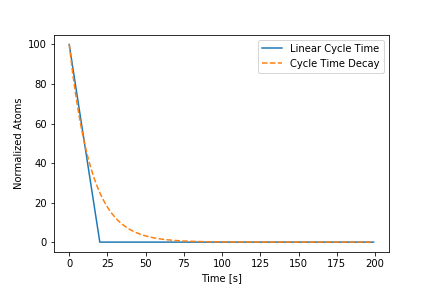
\includegraphics[scale=0.6]{images/Cycle_Time_Decay_example_0.png}
%  \caption{A comparison between a linear 20 second cycle time and the cycle time decay approach.}
%   \label{fig:ctd_examp}
%\end{figure}

%It can be seen in this figure that this approach is accurate in being close to the cycle time, though this accuracy is limited to above approximately 40\% of the atoms. Because fission products are continuously generated though, it is expected to be within the more accurate regions.
%Figure \ref{fig:ctd_examples} shows how the cycle time decay approach fares when accumulation of fission products is incorporated into the problem. 

%\begin{figure}[H]
%  \centering
%  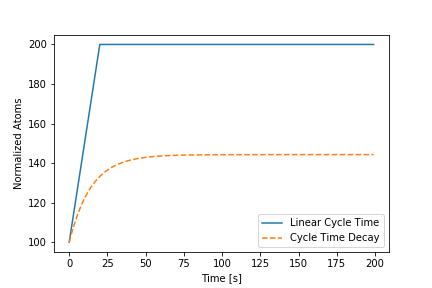
\includegraphics[scale=0.6]{images/Cycle_Time_Decay_example_10.png}
%  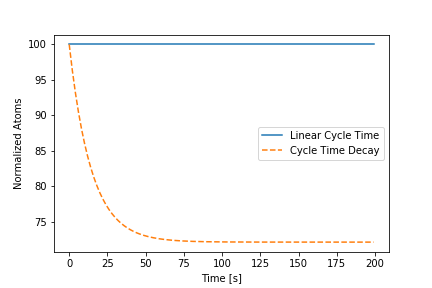
\includegraphics[scale=0.6]{images/Cycle_Time_Decay_example_5.png}
%  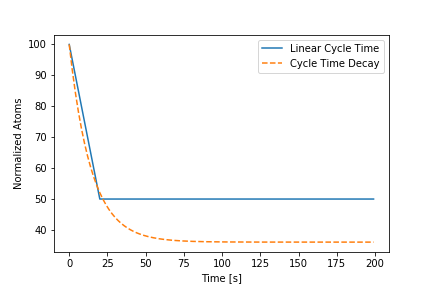
\includegraphics[scale=0.6]{images/Cycle_Time_Decay_example_2.5.png}
%  \caption{Comparison with linear 20 second cycle time and cycle time decay approach for 10, 5, and 2.5 %atoms per second accumulation, respectively.}
%   \label{fig:ctd_examples}
%\end{figure}

%The top plot of Figure \ref{fig:ctd_examples} shows a situation where the accumulation of fission products occurs at a higher rate than the cycle time, leading to a larger steady-state value than initially present. The cycle time decay does not reach the 200 value and instead is lower at 144. The middle plot shows a situation where the accumulation rate matches the cycle time removal rate, the same rate that the linear cycle time would have them removed, resulting in a steady-state value. However, the cycle time decay approach drops to approximately 72 levels off. The bottom plot shows an accumulation which is half the linear cycle time removal rate. These results are somewhat close, though the cycle time decay does not reach the same steady-state value, instead stabilizing around 40 instead of 50. For various accumulation rates ranging from 0.1 to 1 million atoms per second, the steady-state difference comes out to approximately 27.86\% for each. This percent difference also stays the same for different cycle times as well.

An example of implementing this approach for a 30 second cycle time would then have a 15 second reprocessing half-life. This is then converted to a reprocessing constant in the same way that a decay half-life is converted to a decay constant, which is done by plugging these values into Equation \eqref{eq:ctd_2}, resulting in a value of 0.0462 $s^{-1}$.


\subsubsection{SaltProc Cycle Time Decay}

This approach is the same as cycle time decay, but alters for any target which has a cycle time less than the batchwise reprocessing step incorporated by SaltProc. For example, a 3 day cycle time for some target would be treated the same as the standard cycle time decay. However, a cycle time shorter than the 3 day batchwise reprocessing step used by SaltProc for the MSBR has its half-life extended to the SaltProc minimum value of 1.5 days. For example, a 30 second cycle time would instead be treated as a 3 day cycle time, which would result in a half-life of 1.5 days. Plugging in, this would result in a reprocessing constant of 0.462 days$^{-1}$, or 5.348E-6 $s^{-1}$. This is the reprocessing constant for any cycle time which is less than or equal to three days. Additionally, the decay constant is multiplied by the fractional efficiency of the removal used by SaltProc. In most cases the value is 1, but it is roughly 0.91 for xenon and krypton in order to align with Rykhlevskii's results \cite{rykhlevskii_fuel_2020}.

\subsubsection{Cycle Rate}
\label{s:CR}

The cycle rate approach uses a linear approximation such that the inverse of the cycle time is the rate at which material is removed. This is represented by, for example, 10\% removal per second would neglect the efficiency decrease over time and give 100\% removal after 10 seconds. This is calculated by investigating a unit time progression, i.e. 1 second or 1 day. Over this time period, the removal of atoms should be the fractional rate value, which means the final atom count at a time of 1 should be 1 - $f$, where $f$ is the fractional removal rate. This can be seen in Equations \eqref{eq:nat_log_0} and \eqref{eq:nat_log_3}.

First, I start with Equation \eqref{eq:nat_log_0} to define the fraction removed per unit time based on the time units used to define the cycle time.

\begin{equation} \hfill
f = \frac{1}{T_{cyc}}
\hfill\label{eq:nat_log_0} \end{equation}

Next, I define a nuclide Bateman equation with only reprocessing removal considered in Equation \eqref{eq:nat_log_1}.

\begin{equation} \hfill
\frac{dN}{dt} = -\lambda_r N
\hfill\label{eq:nat_log_1} \end{equation}

This equation is then solved for the concentration as a function of time in Equation \eqref{eq:nat_log_1_half}.

\begin{equation} \hfill
N(t) = N_0 e^{-\lambda_r t}
\hfill\label{eq:nat_log_1_half} \end{equation}

After solving, a unit time value is plugged in. After a unit time, the amount of the nuclide remaining should be $(1-f)$, as shown in Equation \eqref{eq:nat_log_2}.

\begin{equation} \hfill
N(t = 1) = (1-f) N_{0}
\hfill\label{eq:nat_log_2} \end{equation}

After plugging in the concentration equation from Equation \eqref{eq:nat_log_1_half} into Equation \eqref{eq:nat_log_2}, Equation \eqref{eq:nat_log_3} is generated.

%\begin{equation} \hfill
%(1-f) N_{0} = N_{0} e^{-\lambda_r (1)}
%\hfill\label{eq:nat_log_2_1} \end{equation}

%\begin{equation} \hfill
%-ln(1-f)  = \lambda_r
%\hfill\label{eq:nat_log_2_5} \end{equation}

%Finally, the reprocessing constant is isolated, resulting in Equation \eqref{eq:nat_log_3}.

\begin{equation} \hfill
\lambda_r = ln\left( \frac{1}{1-f} \right)
\hfill\label{eq:nat_log_3} \end{equation}

%However, the mathematical model actually results in exponential decay in the removal effectiveness due to a decreasing amount of the target to remove. %Figure \ref{fig:cr_examp} shows how this approach compares to the actual exponential decay.

%\begin{figure}[H]
%  \centering
%  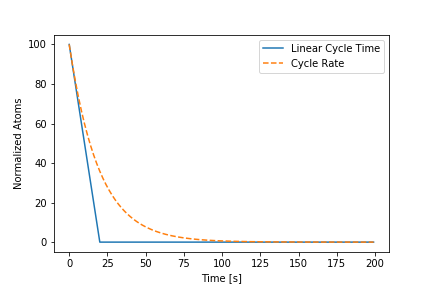
\includegraphics[scale=0.6]{images/Cycle_Rate_example_0.png}
%  \caption{A comparison between a linear 20 second cycle time and the cycle rate approach.}
%   \label{fig:cr_examp}
%\end{figure}

%It can be seen from this figure that the cycle rate approach removes at a rate sufficient to match the cycle time of 20 seconds while there are ~60\% of the atoms present. Once the atom count drops, the removal becomes less effective however, which is physical but makes the model less effective at matching the cycle time. Because the cycle rate approach is used on fission products which are being constantly generated, the difference is expected to be fairly small.

%\begin{figure}[H]
%  \centering
%  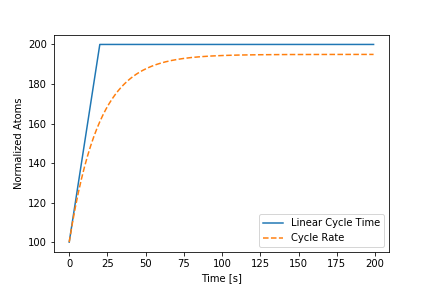
\includegraphics[scale=0.6]{images/Cycle_Rate_example_10.png}
%  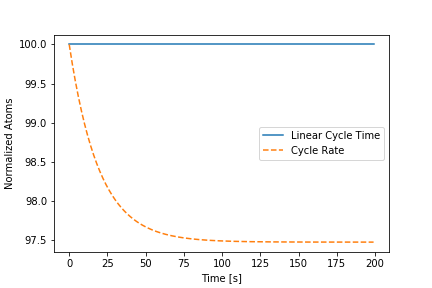
\includegraphics[scale=0.6]{images/Cycle_Rate_example_5.png}
%  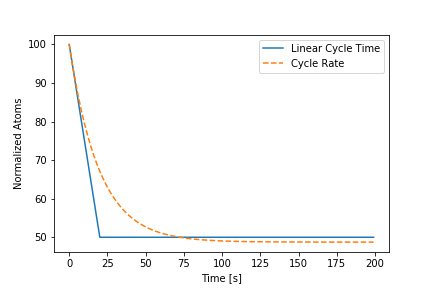
\includegraphics[scale=0.6]{images/Cycle_Rate_example_2.5.png}
%  \caption{Comparison with linear 20 second cycle time and cycle rate approach for 10, 5, and 2.5 atoms %per second accumulation, respectively.}
%   \label{fig:cr_examples}
%\end{figure}



To better clarify the approach, here is an example. A cycle time of 30 seconds would be modeled by taking the inverse, which gives 0.033 $s^{-1}$.
This value is then converted to a reprocessing constant by plugging it into the solved differential equation form shown in Equation \eqref{eq:nat_log_3}, yielding a reprocessing constant of 0.0339 $s^{-1}$.
%This value is then converted to a reprocessing constant by plugging it into the solved differential equation form shown in Equations \eqref{eq:cr_exmp1} and \eqref{eq:cr_eqn}, giving a value of 0.0339 $s^{-1}$.

%\begin{equation} \hfill
%f = \frac{1}{30} = 3.33E\minus2 s^{-1}
%\hfill\label{eq:cr_exmp1} \end{equation}

%\begin{equation} \hfill
%\lambda_{r} = ln\left(\frac{1}{1 - 3.33E\minus2}\right) = 0.0339 s^{-1}
%\hfill\label{eq:cr_eqn} \end{equation}

%The reason this approach is used is two-fold. Firstly, SaltProc v0.3 uses the same linear fractional removal approximation for its batchwise removal, so this same method is employed to better compare the two models. Secondly, due to the mathematical nature of the Decay reprocessing model, 100\% removal only occurs for a reprocessing constant of infinity. This means an approximation must be made. This is also a reasonable approximation since there is constant addition of material, meaning that the exponential line and the linear line are not going to be significantly different.


\subsubsection{SaltProc Cycle Rate}

The SaltProc cycle rate approach is the same as the cycle rate approach, but takes into account the limiting nature of the 3 day batchwise reprocessing step used by SaltProc. For example, a 6 day cycle time target would be modeled the same using the SaltProc cycle rate approach as the standard cycle rate approach. However, anything shorter than 3 days would be modeled differently, since that is the batchwise reprocessing step incorporated by SaltProc for modeling the MSBR. For example, a 30 second cycle time would be analyzed instead as a 3 day cycle time, since SaltProc can only remove 100\% of material after a minimum of 3 days. This means the inverse would be 0.333 $d^{-1}$, or 3.858E-4 $s^{-1}$. Converting to a reprocessing constant gives a value of 3.858E-6 $s^{-1}$. This is the reprocessing constant for any cycle time which is less than or equal to three days. Additionally, the decay constant is multiplied by the fractional efficiency of the removal used by SaltProc. In most cases the value is 1, but it is roughly 0.91 for xenon and krypton in order to align with Rykhlevskii's results \cite{rykhlevskii_fuel_2020}.

\subsubsection{Direct Linear Approach}
\label{s:DL}

Another approach is to directly apply the cycle rate removal rate, which is the inverse of the cycle time, as the reprocessing constant \cite{hombourger_eql0d_2020}. This is referred to as the direct linear approach. This approach is similar to the cycle rate approach, though the derivation for it is slightly different. This can be seen in Equations \eqref{eq:dir_lin_0} through \eqref{eq:dir_lin_10}.%, where Equations \eqref{eq:dir_lin_8} and \eqref{eq:dir_lin_9} uses L'Hôpital's rule.

To start, the derivation begins with the same fractional removal rate as the cycle rate approach in Equation \eqref{eq:dir_lin_0}.

\begin{equation} \hfill
f = \frac{1}{T_{cyc}}
\hfill\label{eq:dir_lin_0} \end{equation}

Then, the Bateman equation for a nuclide with only losses due to reprocessing is solved, with the concentration as a function of time given in Equation \eqref{eq:dir_lin_1_2}.

%\begin{equation} \hfill
%\frac{dN}{dt} = -\lambda_r N
%\hfill\label{eq:dir_lin_1} \end{equation}

\begin{equation} \hfill
N(t) = N_0 e^{-\lambda_r t}
\hfill\label{eq:dir_lin_1_2} \end{equation}

This equation can be rewritten as multiplying the previous concentration by a value dependent on the time step, as shown in Equation \eqref{eq:dir_lin_2}.

\begin{equation} \hfill
N_{cur} = N_{prev} e^{-\lambda_r \Delta t}
\hfill\label{eq:dir_lin_2} \end{equation}

In addition, after each step, the fractional removal is applied over that time step, allowing for the current concentration to be calculated as shown in Equation \eqref{eq:dir_lin_3}.

\begin{equation} \hfill
N_{cur} = (1 - \Delta t f) N_{prev}
\hfill\label{eq:dir_lin_3} \end{equation}

Equations \eqref{eq:dir_lin_2} and \eqref{eq:dir_lin_4} are then set equal to each other, yielding Equation \eqref{eq:dir_lin_4}.

\begin{equation} \hfill
(1 - \Delta t f) N_{prev} = N_{prev} e^{-\lambda_r \Delta t}
\hfill\label{eq:dir_lin_4} \end{equation}

This equation is simplified to the form shown in Equation \eqref{eq:dir_lin_5}.

\begin{equation} \hfill
-ln\left((1 - \Delta t f)\right) = \lambda_r \Delta t
\hfill\label{eq:dir_lin_5} \end{equation}

Solving for $\lambda_r$ yields Equation \eqref{eq:dir_lin_6}.

\begin{equation} \hfill
\lambda_r = \frac{-ln\left((1 - \Delta t f)\right)}{\Delta t}
\hfill\label{eq:dir_lin_6} \end{equation}

Instead of seeking the reprocessing constant for a unit time step as found using the cycle rate approach, I instead seek the reprocessing constant as the time step approaches zero as shown in Equation \eqref{eq:dir_lin_7}.

\begin{equation} \hfill
\lambda_r = lim_{\Delta t \to 0} \frac{-ln\left((1 - \Delta t f)\right)}{\Delta t}
\hfill\label{eq:dir_lin_7} \end{equation}

Because this results in a fraction of zero over zero, as shown in Equation \eqref{eq:dir_lin_8}, I use L'Hôpital's rule to change to the form shown in Equation \eqref{eq:dir_lin_9}.

\begin{equation} \hfill
\lambda_r = \frac{0}{0}
\hfill\label{eq:dir_lin_8} \end{equation}

\begin{equation} \hfill
\lambda_r = lim_{\Delta t \to 0} \frac{f}{1-f\Delta t}
\hfill\label{eq:dir_lin_9} \end{equation}

This form can then be directly solved, yielding the reprocessing constant equation shown in Equation \eqref{eq:dir_lin_10}.

\begin{equation} \hfill
\lambda_r = f = \frac{1}{T_{cyc}}
\hfill\label{eq:dir_lin_10} \end{equation}

These equations follow a similar path to the cycle rate approach, but instead of using the linear approximation value after a unit time step, this approach generates the reprocessing constant while implementing the linear approximation as the time step goes to zero.

The differences between the cycle rate and direct linear reprocessing constants can be seen in Table \ref{tab:repr_decay_view}, where for longer cycle times, the difference is negligible, but for shorter cycle times, the difference becomes larger. However, since extremely short cycle times are not realistically practical, the two approaches are approximately equivalent. Overall, the direct linear approach is more numerically stable, however, since it does not have asymptotic behavior until reaching a cycle time of zero seconds, whereas the cycle rate method has asymptotic behaviour for a one second cycle time. This can be seen from the form of the equations for the reprocessing constants and in Figure \ref{fig:dl_cr_asymptotic}, which displays how the reprocessing constants vary for various cycle times. The asymptotic behaviour for a zero second cycle time is not an issue because as the cycle time goes to zero, that would mean that the target is removed over zero seconds. This means an infinite removal rate would be physical. Additionally, there are no negative cycle times, meaning the value is only approached from the positive side and behaves as physically expected. Realistically, reprocessing scheme cycle times are longer than the order of seconds, which means for most practical use cases these two approaches are interchangable.

\begin{table}[H]
\renewcommand{\arraystretch}{1.25}
\caption{Subset of Decay Reprocessing Approaches}
\label{tab:repr_decay_view}
\begin{center}
\begin{tabular}{ c | c | c | c | c }
 \hline
 Cycle Time & Removal Rate [$s^{-1}$] & CR $\lambda_{r}$ [$s^{-1}$] & DL $\lambda_{r}$ [$s^{-1}$] & $\Delta \lambda_{r}$\\
 \hline
 \hline
 3 d & 3.86E-6 & 3.86E-6 & 3.86E-6 & 7.44E-12\\
 20 s & 0.05 & 5.13E-2 & 5.00E-2 & 1.29E-3\\
 5 s & 0.2 & 2.23E-1 & 2.00E-1 & 2.31E-2\\
 2 s & 0.5 & 6.93E-1 & 5.00E-1 & 1.93E-1\\
 1 s & 1 & - & 1 & -\\
 \hline
\end{tabular}
\end{center}
\end{table}

\begin{figure}[H]
  \centering
  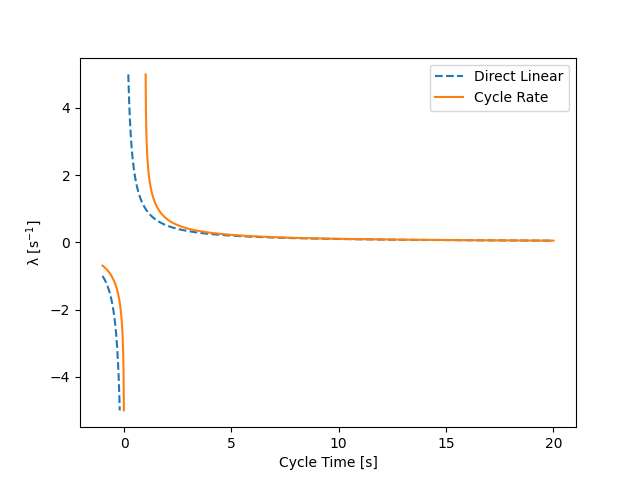
\includegraphics[scale=0.7]{images/dl_cr_asymptote.png}
  \caption{An illustrated comparison of the direct linear and cycle rate reprocessing constants for different cycle times.}
   \label{fig:dl_cr_asymptotic}
\end{figure}

Because the shortest cycle time for the MSBR is 20 seconds, this shows that the cycle rate and direct linear approaches are roughly equivalent for this reprocessing scheme.

%Figure \ref{fig:dl_cr_compare_linear} shows the implementation of both methods for an example nuclide with a cycle time of CYCLE TIME and an accumulation rate of ACCUMULATION RATE. It can be seen from this figure how the direct linear and cycle rate approaches differ in modeling of the same isotope.

%\begin{figure}[H]
%  \centering
%  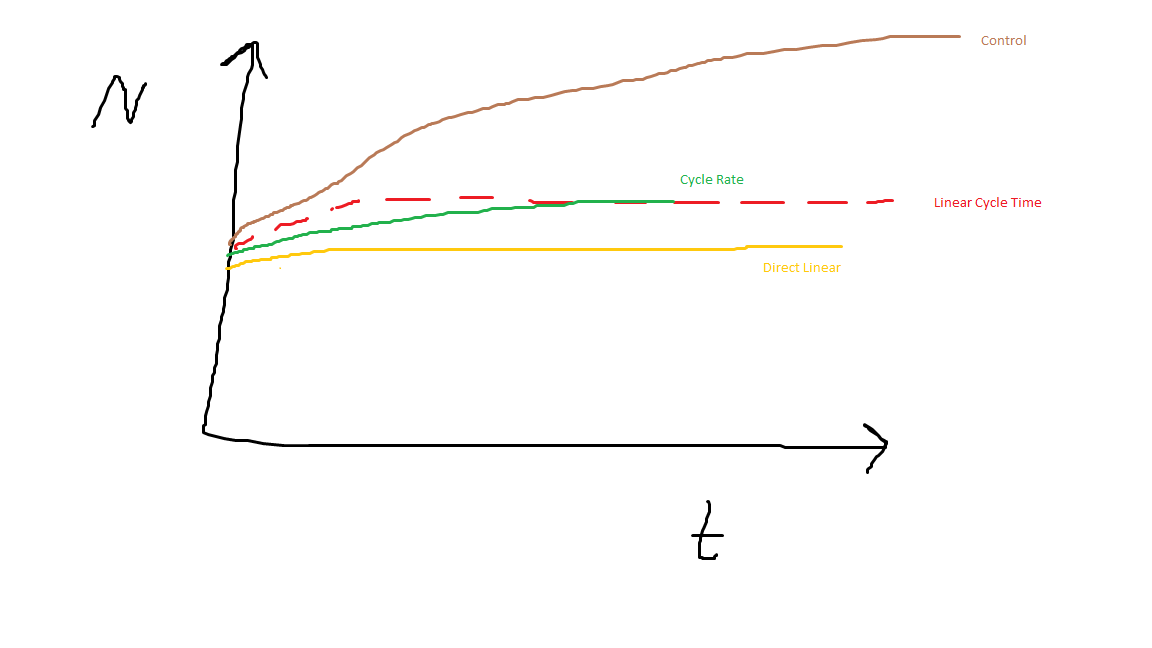
\includegraphics[scale=0.25]{images/direct_linear_compare.png}
%  \caption{A comparison of the direct linear and cycle rate approaches for a particular element with a %given accumulation rate and cycle time(s).}
%   \label{fig:dl_cr_compare_linear}
%\end{figure}

\subsubsection{SaltProc Direct Linear Approach}

The SaltProc direct linear approach is the same as the direct linear approach, but takes into account the limiting nature of the 3 day batchwise reprocessing step used by SaltProc. For example, a 6 day cycle time target would be modeled the same using the SaltProc direct linear approach as the standard direct linear approach. However, anything shorter than 3 days would be modeled differently, since that is the batchwise reprocessing step inocorporated by SaltProc for modeling the MSBR. For example, a 30 second cycle time would be analyzed instead as a 3 day cycle time, since SaltProc can only remove 100\% of material after a minimum of 3 days. This means the inverse would be 0.333 days$^{-1}$, or 3.858E-4 $s^{-1}$. Converting to a reprocessing constant gives a value of 3.858E-6 $s^{-1}$. This is the reprocessing constant for any cycle time which is less than or equal to three days. Additionally, the decay constant is multiplied by the fractional efficiency of the removal used by SaltProc. In most cases the value is 1, but it is roughly 0.91 for xenon and krypton in order to align with Rykhlevskii's results \cite{rykhlevskii_fuel_2020}.
%The SaltProc direct linear approach follows the same trend as the other SaltProc-based modified approaches. This includes changing the smallest time scale to 3 days and altering the fractional removal values of xenon and krypton.

\subsubsection{Decay Approaches Summary}



\begin{figure}[H]
  \centering
  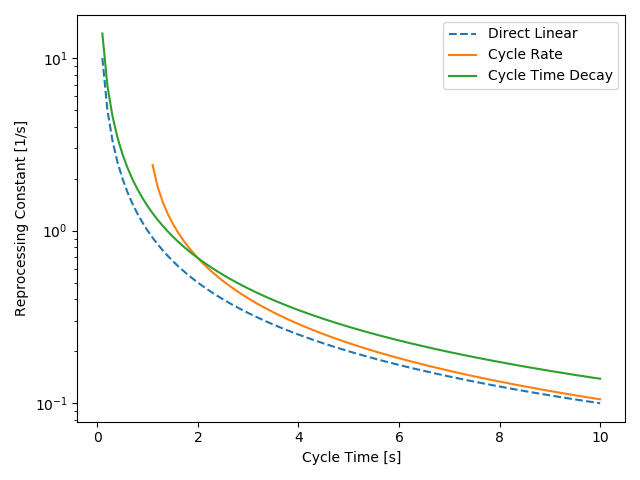
\includegraphics[scale=0.7]{images/cont-compare-cycles.png}
  \caption{Plot of how reprocessing constants for different approaches vary with cycle time.}
   \label{fig:repr_cnst}
\end{figure}

Figure \ref{fig:repr_cnst} shows how the reprocessing constants for the different approaches vary as a function of cycle time.
This figure includes the three different continuous decay based methods for reprocessing as a function of various cycle times. From the figure, it can be seen that the cycle rate method does not have results for cycle times less than or equal to 1 second, which is a significant weakness of the method since physical processes could exist with a cycle time in that range. The other two methods provide results down to a 0 second cycle time, which allows full coverage of possible cycle time values.

The direct linear method behaves similarly to the cycle time decay method during small cycle times and the cycle rate method for longer cycle times. This is due to the general form of the equations for each, where at small cycle times the inverse cycle time relationship with the cycle time decay method dominates, while at larger cycle times the cycle rate log of the inverse term matches more closely.


Table \ref{tab:repr_decay_view_full} shows all the different decay based continuous reprocessing approaches for various cycle times. From this table, it can be seen that the direct linear and cycle rate methods are very close, while the cycle time decay method is off by a small amount at all cycle times. In terms of the SaltProc variants, the main difference is the fact that the cycle times below three days have been assigned the reprocessing constant of the three day cycle time.

\begin{table}[H]
\renewcommand{\arraystretch}{1.25}
\caption{Full Set of Decay Reprocessing Approaches for Various Cycle Times}
\label{tab:repr_decay_view_full}
\begin{center}
\begin{tabular}{ c | c | c | c | c }
 \hline
 Method & $T_{cyc} = 1 s$ & $T_{cyc} = 20 s$ & $T_{cyc} = 3 d$ & $T_{cyc} = 50 d$\\
 \hline
 \hline
 DL & 1 & 5.00E-2 & 3.86E-6 & 2.31E-7\\
 CR & - & 5.13E-2 & 3.86E-6 & 2.31E-7\\
 CTD & 1.39 & 6.93E-2 & 5.35E-6 & 3.21E-7\\
 \hline
 SPDL & 3.86E-6 & 3.86E-6 & 3.86E-6 & 2.31E-7\\
 SPCR & 3.86E-6 & 3.86E-6 & 3.86E-6 & 2.31E-7\\
 SPCTD & 5.35E-6 & 5.35E-6 & 5.35E-6 & 3.21E-7\\
 \hline
\end{tabular}
\end{center}
\end{table}

The values shown in Table \ref{tab:repr_decay_view_full} for the SaltProc-type continuous methods are based on the cycle times given from the Robertson report, which matches what is used in the bulk SaltProc, version 0.1, results. The steady SaltProc results, verson 0.3, do not use these exact values \cite{robertson_conceptual_1971, rykhlevskii_advanced_2018}. The differences in steady SaltProc are as follows: xenon has 91.2\% removal over three days instead of 100\%, krypton has 91.5\% removal over three days instead of 100\%, protactinium has 9.5\% removal over three days instead of 100\%, and the discard has a removal of 0.9\% over three days instead of 0.09\%. %Check Pa, SaltProc actually using 9.5%?????????

%WHICH IS THE MORE ACCURATE APPROACH AMONG THE THREE (There isn't a way to validate this without more information on how cycle time is generated. Perhaps if instead we find data for molten salt reprocessing and compare against that it might be useful?) (Maybe check average net atoms for steady and bulk batch and compare, then maybe check a comparison of net atoms at 1/2 cycle time and cycle time, etc.)

%CITE "Liquid Fuel Molten Salt Reactors for Thorium Utilization" This paper uses bulk batchwise reprocessing

%INCLUDE PLOT OF N(t) FOR DIFFERENT CYCLE TIMES WHERE ONLY INITIAL MASS AND REPROCESSING ARE CONSIDERED. (direct linear AND cycle rate ARE THE SAME FOR LARGE CYCLE TIMES)

%REPLICATE ATOMS OVER TIME PLOTS FOR DIFFERENT MODELS AND DIFFERENT ACCUMULATION RATES TO SEE HOW STEADY-STATE VALUES COMPARE.

\subsection{Step Reprocessing Approach}

The Step reprocessing method implemented in Serpent2 is mathematically very similar to the Decay model, but instead of updating continuously in time, it instead is updated during new depletion steps. In this manner, it could be considered a mix between the Constant method and the Decay method. This is because over a single depletion step, it is a constant added or subtracted from the Bateman equation, while over many depletion steps, it follows the same exponential decay form of the Decay method.

This particular method is not useful for extracting fission products, and is not needed for constant feed rates since that can be modeled using the Decay method. This method could be useful for inducing a step drop in feed rate, though this would require running only a single depletion step until the drop occurred. Additionally, this drop could be simulated by running the Decay method and reducing the reprocessing constant. This would allow for flexibility in the distribution of depletion steps as well without having to worry about changing the behaviour of the reprocessing functionality. 

Another potential issue with the Step method is that the depletion step can last long enough that the constant mass removal causes the mass to go negative. However, Serpent2 will cease running if this occurs. The Decay method does not mathematically allow for negative mass, the Constant method does not conserve mass, and the Step method stops running once there is negative mass.

The main potential use of the Step reprocessing may be for movement of material at a set rate. This could be implemented by writing a script to check the current number of atoms of the target and adjusting the reprocessing rate accordingly. However, for the MSBR, this form of reprocessing is not necessary, and is thus not implemented.

\section{Mass Balancing}
\label{s:mass-bal-meth}

One of the useful features of batchwise reprocessing is that the net mass of the core can be balanced by adjusting the feed rates to provide the same amount into the core that is lost. Alternative methods also exist, such as removing excess mass or increasing the volume \cite{ridley_method_2017}. SaltProc version 0.1 does not account for mass balancing but maintains a constant thorium mass, whereas SaltProc version 0.3 has the feed rates set to maintain mass. Mass balancing is particularly important in Serpent2 due to the way masses in Serpent2 are handled.

In Serpent2, an increase in mass does not affect volume, but instead increases the density of that isotope in the material accordingly. This affects macroscopic cross section calculations, and can lead to variation in results if not accounted for, since in reality volumetric expansion could be assumed. Though there are several methods to handle mass balancing with a batch method, it not currently continuously possible in Serpent2.

In order to balance the mass in Serpent2 continuously, one approach could be to iteratively perform depletion calculations while updating feed rates until a balanced mass is found while also minimizing some other parameter, such as net mass of material added. However, the current reprocessing options available in Serpent2 only allow for pseudo-constant and decaying feed rates over the depletion step. With those two feed types available, it is not possible to have a constant mass balance.

It is possible to have the masses at the end of each depletion step remain constant, but this does not handle mass fluctuations during depletion. It does, however, solve the issue of the density variation causing a difference in cross sections.

Overall, if the net mass difference is sufficiently small, it does not have to be considered since the results would not be significantly impacted. To check this for the MSBR, I will use an illustrative example. To determine the maximum possible increase in density, the mass loss due to fission and reprocessing is neglected, and only mass addition from the thorium feed rate is considered. The uranium feed is not added because it is equivalent to the protactinium removal, so it would have a negligible impact on net mass. 

\begin{equation} \hfill
\Delta m = \Dot{m}_{feed} \Delta t \approx (2.5)(6000) = 15,000 kg
\hfill\label{eq:m_gain} \end{equation}

It can be seen in Equation \eqref{eq:m_gain} that the net mass gain for an average feed rate of 2.5 kilograms per day over 6000 days is 15,000 kg \cite{rykhlevskii_fuel_2020, betzler_molten_2017} while operating at nominal power of 2250 MW \cite{robertson_conceptual_1971}. This does seem to be a very large value, but the importance of the mass in the depletion calculation is primarily in how it affects cross sections, which means that the impact on the overall thorium density is important. The thorium density is 1.46 grams per cubic centimeter, and the net volume is approximately 48.71 cubic meters. The density with the added mass is calculated using Equation \eqref{eq:new_rho}.

\begin{equation} \hfill
\rho_f = \frac{m_0 + \Delta m}{V} = \frac{(4.871E7 \left[cm^3 \right])(1.45919E\minus3 \left[ \frac{kg}{cm^3} \right]) + (15,000 \left[ kg \right])}{4.871E7 \left[ cm^3 \right]} 
\hfill\label{eq:new_rho} \end{equation}

The final density comes out to be 1.767 grams per cubic centimeter, which is a percent difference of ~21\%. Although this is an upper bound on the mass difference, a 21\% difference in the expected cross section would result in significant error in the results. Therefore, since it is possible for the mass balancing to have an impact, it should be investigated to ensure the mass balancing is not impacting the results in any unexpected manner.

%DIFFERENT FEED RATE VARIANTS IMPLEMENTED

%MSBR MASS BALANCE BATCH AND CONTINUOUS


%\section{Uncertainty}

%SHANNON ENTROPY

%STOCHASTIC ERROR VS ACTUAL DIFFERENCE IN RESULTS

%DEPLETION ERROR BUILDUP

%\section{Continuous Reprocessing Implementation}

\section{Effects of Delayed Neutrons on Depletion}

Delayed neutrons have a softer energy spectrum and drift along with the movement of the fuel salt in a fluid fueled molten salt reactor. This means that the delayed neutron precursors, of which some fraction leave the core and some move to less neutron important regions, have the potential to alter the depletion results of the MSBR model.

However, it has been shown by Zhou et al. that for the MSBR, the delayed neutron precursor drift has a negligible impact on depletion results \cite{zhou_fuel_2018}. Although Zhou et al. have shown this, it is still worth considering the maximum possible effect delayed neutron precursors could have on depletion results. In order to determine this, the Serpent2 functionality of disabling delayed neutrons is employed \cite{leppanen_serpent_2015}. Using this method, two different models are generated of the MSBR. The first is one in which the delayed neutron precursors are evenly distributed within the core, which is the model implemented by SaltProc and this work \cite{rykhlevskii_modeling_2019}. The second model is one in which delayed neutrons no longer exist. This is beyond the greatest effects the delayed neutron precursor drift could have on depletion, so the absolute maximum effect of delayed neutron precursors on depletion results can be determined.

Because the delayed neutron precursors are fission products or come from the decay of fission products, depletion must be performed. For reprocessing, the average feed rate from SaltProc is used with continuous direct linear reprocessing, while direct linear reprocessing is used for fission product removal. 

I investigated the impact on $k_{eff}$, and I determined that the delayed neutrons from fission products add roughly 20 pcm to $k_{eff}$ after 6,000 days of operation, which is roughly steady state operation. 
This was determined by running the simulation with and without delayed neutrons enabled and comparing the $k_{eff}$ values.
I also compared the masses of various isotopes, such as uranium-235 and thorium-232, though no statistically significant difference was found. Therefore, the net impact of delayed neutrons from fission product precursors appears to be negligible on the depletion results in this work, which agrees with the results from Zhou et al.

%Figure \ref{fig:keff_compare} shows how the multiplication factors evolve over time. The final difference between the two values is FINALDIFF.

%\begin{figure}[H]
%  \centering
%  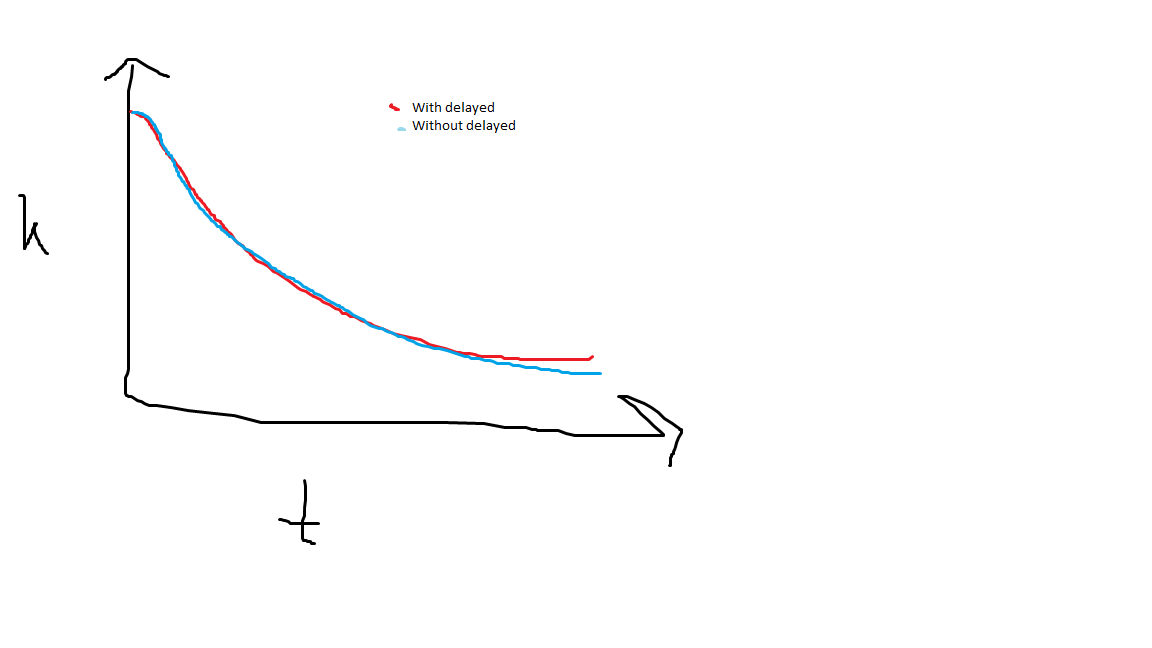
\includegraphics[scale=0.7]{images/keff_dnp_compare.png}
%  \caption{Comparison of $k_{eff}$ over time with and without delayed neutrons.}
%   \label{fig:keff_compare}
%\end{figure}

%PLOT OF SPECTRUMS WITH AND WITHOUT DELAYED NEUTRONS

%TABLE OF IMPORTANT ISOTOPE CONCENTRATIONS FOR WITH AND WITHOUT





% Toggle remove this for debugging
%\nocite{*}


